\documentclass[conference]{IEEEtran}
\IEEEoverridecommandlockouts
\usepackage{amsmath,amssymb,siunitx,xcolor,tikz,float,cite}
\usepackage[T1]{fontenc}
\usepackage{microtype,graphicx,booktabs,array,multirow}
\usepackage[american]{circuitikz}
\usepackage[hidelinks]{hyperref}
\usetikzlibrary{arrows.meta,calc}
\tikzset{every node/.append style={inner sep=1.5pt}}
\graphicspath{{figures/}}
\setlength{\tabcolsep}{3pt}
\renewcommand{\arraystretch}{1.08}
\setlength{\textfloatsep}{10pt plus 2pt minus 2pt}
\renewcommand{\topfraction}{0.9}\renewcommand{\dbltopfraction}{0.9}
\renewcommand{\textfraction}{0.05}\renewcommand{\floatpagefraction}{0.85}
\newcommand{\Vin}{V_{\mathrm{IN}}}\newcommand{\Vout}{V_{\mathrm{OUT}}}
\newcommand{\Cout}{C_{\mathrm{OUT}}}\newcommand{\Cgd}{C_{gd}}
\hypersetup{pdftitle={NCM-LDO: a neutralized current-mode LDO for an on-chip PLL supply in 180 nm CMOS},pdfauthor={Garaga Karthikeya}}

\begin{document}
\title{Design of a Neutralized Current-Mode LDO\\for an On-Chip PLL Supply in 180-nm CMOS}
\author{\IEEEauthorblockN{Garaga Karthikeya (IMT2024073)}
\IEEEauthorblockA{Course project report, Analog CMOS VLSI Design\\
International Institute of Information Technology Bangalore (IIIT Bangalore)\\
November 2026}}
\maketitle

\begin{abstract}
This report describes the design of a low-dropout regulator (LDO) that turns a shared, noisy 1.8-V rail into a clean 1.4-V supply for an on-chip phase-locked loop (PLL) in a 180-nm CMOS process. A conventional LDO cannot reject supply ripple above its loop bandwidth, so its power-supply rejection (PSRR) has a hump in the 1--100-MHz range, exactly where a voltage-controlled oscillator is sensitive. I designed a \emph{neutralized current-mode} LDO (NCM-LDO): the pass transistor is a 100$\times$ current-mirror copy of a reference device whose drain is held at $\Vout$, which cancels the pass device's $g_m$ and $g_{ds}$ ripple paths, and a 1-pF capacitor neutralizes the gate--drain capacitance current that the mirror would otherwise multiply by 100. All devices were sized with the $g_m/I_D$ method from the course techplots. In LTspice simulation (typical models, 27$^\circ$C) the regulator achieves $-31.3$~dB worst-case PSRR from 10~Hz to 10~GHz over 1.71--1.89~V and 8--10~mA, with 289~$\mu$A quiescent current, exactly 1~nF of on-chip capacitance, 25-mV dropout, at least 48.9$^\circ$ phase margin from no load to full load, 18.4~nV/$\sqrt{\rm Hz}$ output noise at 1~MHz and $\pm$17~mV error for an 8$\leftrightarrow$10-mA load step. Because both amplifiers are powered from the output, the regulator cannot start by itself; a four-transistor start-up kick brings it up cleanly from 0~V for supply ramps from 0.1 to 100~$\mu$s.
\end{abstract}

\section{Introduction and Specifications}
A PLL's voltage-controlled oscillator (VCO) converts any ripple on its supply into frequency modulation, which shows up as jitter. On a SerDes chip the PLL usually shares the 1.8-V rail with noisy digital and I/O circuits, so the PLL gets its own on-chip LDO. Because the ripple can be anywhere from switching-regulator frequencies (100~kHz) to digital clock harmonics (hundreds of MHz), I wanted the PSRR to be good over the \emph{whole} band, not only at low frequency.

Table~\ref{tab:specs} lists the specifications I set and how hard each one is. PSRR was originally $-40$~dB; reaching it with the topology in this report would cost about 770~$\mu$A, so I relaxed it to $-30$~dB to stay inside the 300-$\mu$A budget. The tight one is headroom: 1.71~V in and 1.40~V out leaves only 310~mV, so there is no room for a series isolating transistor and the pass device alone must handle dropout.

\begin{table}[!t]
\centering
\caption{Specifications and how aggressive each one is}
\label{tab:specs}
\footnotesize
\begin{tabular}{@{}lcl@{}}
\toprule
Parameter & Target & Class \\
\midrule
Input $\Vin$ & 1.8 V ($\pm$5\%) & Shared, noisy rail \\
Output $\Vout$ & 1.4 V $\pm$1\% & Moderate \\
Load current & 8--10 mA, stable 0--10 mA & Moderate \\
Headroom at 1.71 V & 310 mV & Aggressive \\
PSRR, 10 Hz--10 GHz & $\le -30$ dB worst case & Aggressive \\
Quiescent current & $\le$ 300 $\mu$A & Moderate \\
Total capacitance & $\le$ 1 nF, fully on chip & Aggressive \\
Load step 8$\leftrightarrow$10 mA, 10 ns & $\pm$20 mV & Moderate \\
Output noise at 1 MHz & $\le$ 20 nV/$\sqrt{\rm Hz}$ & Moderate \\
Phase margin, 0--10 mA & $\ge 45^\circ$ & Relaxed \\
\bottomrule
\end{tabular}
\end{table}

All simulations use LTspice with the course 180-nm models (BSIM3, typical corner, 27$^\circ$C) and ideal reference and bias sources. The design, the spreadsheet with the hand calculations, the scripts and the LTspice schematic are in the project repository.

\section{Why a Conventional LDO Has a PSRR Hump}
In a PMOS LDO, supply ripple $v_{in}$ reaches the output through the pass transistor in three ways:
\begin{equation}
i_{\rm leak} = g_m\,(v_{in}-v_g) + g_{ds}\,(v_{in}-v_{out}) + sC_{gd}\,(v_g-v_{out}).
\label{eq:leak}
\end{equation}
At low frequency the loop gain suppresses the resulting output error. Above the loop's unity-gain frequency $f_u$ nothing suppresses it, and the output ripple is roughly $i_{\rm leak}\,Z_{\rm out}$, where $Z_{\rm out}\approx 1/(s\Cout)$ only becomes small at very high frequency. In between, the PSRR rises to a peak: the \emph{hump}. With only $\sim$1~nF available on chip, $Z_{\rm out}$ is still several ohms at 10~MHz, so the hump is large.

Fig.~\ref{fig:conv} shows this for a conventional LDO with the same pass device (5-transistor OTA, Miller-type gate capacitor, 100~$\mu$A, 839~pF): the PSRR is $-60$~dB at DC but climbs to about 0~dB at 3.5~MHz. The pass device at $g_m/I_D=10$ has $g_m r_o\approx 22$, so if its gate stops following $\Vin$, the ripple reaches the output with a gain of $g_m(r_o\parallel R_L)\approx +19$~dB. To get broadband PSRR on chip, the leak in (\ref{eq:leak}) has to be \emph{cancelled}, not filtered. Published high-PSRR LDOs do this by feeding a copy of the ripple into the pass gate~\cite{elnozahi,choe} or body~\cite{lim}; this design cancels each term inside the pass stage instead.

\begin{figure}[!t]
\centering
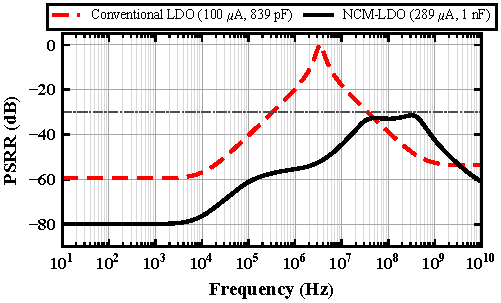
\includegraphics[width=\columnwidth]{psrr_conventional}
\caption{PSRR at 1.8~V, 10~mA: conventional LDO with the same pass device versus the NCM-LDO. The dash-dot line marks the $-30$-dB specification.}
\label{fig:conv}
\end{figure}

\section{Proposed Topology: the NCM-LDO}
Fig.~\ref{fig:concept} shows the idea and Fig.~\ref{fig:schematic} the complete circuit. Each term of (\ref{eq:leak}) is cancelled separately.

\begin{figure}[!t]
\centering
\resizebox{\columnwidth}{!}{% Concept: the three leak paths and what cancels each
\begin{circuitikz}[line width=.6pt,font=\fontsize{8}{9}\selectfont]
\ctikzset{bipoles/length=.85cm,transistors/scale=1.0,tripoles/mos style/arrows,tripoles/pmos style/nocircle}
\draw[line width=.85pt] (0,4.2) node[left]{$V_{\rm IN}$} -- (6.2,4.2);
\node[pmos,xscale=-1] (mref) at (2.2,3.2) {};
\node[pmos] (mp) at (5.0,3.2) {};
\draw (mref.S) -- (2.2,4.2); \draw (mp.S) -- (5.0,4.2);
\draw (mref.G) -- (mp.G); \coordinate (g) at (3.6,3.2); \fill (g) circle(1pt);
\node[above] at (g){$g$};
\coordinate (r) at (2.2,2.2); \draw (mref.D) -- (r); \fill (r) circle(1pt);
\draw (1.1,4.2) to[C,l_=$C_N$] (1.1,2.2) -- (r); \fill (1.1,4.2) circle(1pt); \fill (2.2,4.2) circle(1pt);
\node[pmos] (mc) at (2.2,1.3) {};
\draw (mc.S) -- (r);
\draw (mc.D) -- (2.2,.3) coordinate(gb) -- (3.6,.3) -- (g); \fill (gb) circle(1pt);
\draw (gb) to[I,l_=$I_{\rm REF}$] (2.2,-1.0) node[ground]{};
\coordinate (vo) at (5.0,2.0); \draw (mp.D) -- (vo) -- (6.2,2.0) node[right]{$V_{\rm OUT}$}; \fill (vo) circle(1pt);
% tracking amplifier as an op-amp: + = VOUT, - = r, output -> Mc gate
\node[op amp,scale=.55] (oa) at (.15,1.3) {};
\draw (oa.out) -- (mc.G);
\draw (oa.-) -- ++(-.15,0) node[left]{$r$};
\draw (oa.+) -- ++(-.15,0) node[left]{$V_{\rm OUT}$};
\node[left] at (1.95,3.55){$1$}; \node[right] at (5.25,3.55){$N$};
\node[right] at (2.4,1.3){M$_{\rm C}$};
\node[font=\fontsize{6.5}{7}\selectfont,align=left,anchor=west] at (5.55,3.1){(1) $g_m$: $g$ follows $V_{\rm IN}$\\(2) $g_{ds}$: $r=V_{\rm OUT}$\\(3) $C_{gd}$: $C_N$ into $r$};
\end{circuitikz}
}
\caption{Idea of the NCM-LDO. M$_{\rm PASS}$ is an $N=100$ copy of M$_{\rm REF}$; the tracking amplifier holds the reference drain $r$ at $\Vout$ through cascode M$_{\rm C}$, and $C_N$ supplies the gate--drain current. Numbers (1)--(3) refer to the leak terms of (\ref{eq:leak}).}
\label{fig:concept}
\end{figure}

\begin{figure*}[!t]
\centering
\resizebox{\textwidth}{!}{% Full NCM-LDO schematic (values: Table II and design.py)
\begin{circuitikz}[line width=.6pt,font=\fontsize{8}{9}\selectfont]
\ctikzset{bipoles/length=.9cm,transistors/scale=1.0,tripoles/mos style/arrows,tripoles/pmos style/nocircle}
% ---------------- error amplifier (supply = VOUT) ----------------
\draw[line width=.85pt] (-1.2,6.4) node[left]{$V_{\rm OUT}$} -- (5.2,6.4);
\draw (-.7,6.4) to[R,l_=$R_T$] (-.7,3.9) coordinate(fb) to[R,l_=$R_B$] (-.7,-.5);
\draw (.2,6.4) to[C,l=$C_{FF}$] (.2,3.9) -- (fb);
\fill (fb) circle(1pt); \fill (-.7,6.4) circle(1pt); \fill (.2,6.4) circle(1pt);
\node[below] at (-.25,3.9){FB};
\draw (3.2,6.4) to[I,l=$I_{T}$] (3.2,5.0) coordinate(tp);
\node[pmos] (pi1) at (2.4,4.2) {};
\node[pmos,xscale=-1] (pi2) at (4.0,4.2) {};
\draw (pi1.S) |- (tp) -| (pi2.S); \fill (tp) circle(1pt);
\draw (pi1.G) -- ++(-.25,0) node[left]{$V_{\rm REF}$};
\draw (pi2.G) -- ++(.25,0) node[right]{FB};
\node[nmos,xscale=-1] (nl1) at (2.4,1.4) {};
\node[nmos] (nl2) at (4.0,1.4) {};
\draw (pi1.D) -- (nl1.D); \draw (pi2.D) -- (nl2.D);
\draw (nl1.G) -- (nl2.G); \draw (nl1.G) ++(.25,0) coordinate(mg) |- (2.4,2.5); \fill (mg) circle(1pt); \fill (2.4,2.5) circle(1pt);
\draw (nl1.S) -- (2.4,-.5); \draw (nl2.S) -- (4.0,-.5);
\coordinate (od) at (4.0,2.6); \fill (od) circle(1pt);
\draw (od) -- (5.2,2.6) to[R,l=$R_Z$] (5.2,1.0) to[C,l=$C_Z$] (5.2,-.5);
\fill (5.2,2.6) circle(1pt);
\draw (5.2,2.6) -- (5.9,2.6) node[right]{OD};
\node at (1.75,4.8){M$_{\rm PI1}$}; \node at (4.65,4.8){M$_{\rm PI2}$};
\node[left] at (2.15,.95){M$_{\rm NL1}$}; \node[right] at (4.25,.95){M$_{\rm NL2}$};
% ---------------- mirror power stage and driver ----------------
\draw[line width=.85pt] (6.9,6.4) node[left]{$V_{\rm IN}$} -- (11.0,6.4);
\node[pmos,xscale=-1] (mref) at (8.6,5.4) {};
\node[pmos] (mp) at (10.6,5.4) {};
\draw (mref.S) -- (8.6,6.4); \draw (mp.S) -- (10.6,6.4);
\draw (mref.G) -- (mp.G); \coordinate (g) at (9.55,5.4); \fill (g) circle(1pt);
\draw (9.55,6.4) to[R,l_=$R_G$] (g);
\fill (8.6,6.4) circle(1pt); \fill (9.55,6.4) circle(1pt); \fill (7.4,6.4) circle(1pt);
\coordinate (r) at (8.6,4.4);
\draw (mref.D) -- (r);
\draw (7.4,6.4) to[C,l_=$C_N$] (7.4,4.4) -- (r); \fill (r) circle(1pt);
\node[above left] at (r){$r$};
\node[pmos] (mc) at (8.6,3.5) {};
\draw (mc.S) -- (r);
\draw (mc.G) -- ++(-.3,0) node[left]{GC};
\node[nmos] (mcn) at (8.6,1.75) {};
\draw (mc.D) -- (mcn.D);
\coordinate (gg) at (8.6,2.6); \fill (gg) circle(1pt);
\draw (gg) -- (9.55,2.6) -- (g);
\node[right] at (9.55,3.4){$g$};
\draw (mcn.G) -- ++(-.3,0) node[left]{$V_{\rm CN}$};
\node[nmos] (md) at (8.6,.35) {};
\draw (mcn.S) -- (md.D);
\draw (md.G) -- ++(-.3,0) node[left]{OD};
\draw (md.S) -- (8.6,-.5);
\node[left] at (8.35,5.85){M$_{\rm REF}$}; \node[right] at (10.85,5.85){M$_{\rm PASS}$};
\node[right] at (8.85,3.5){M$_{\rm C}$}; \node[right] at (8.85,1.75){M$_{\rm CN}$}; \node[right] at (8.85,.35){M$_{\rm DRV}$};
% output
\coordinate (vo) at (10.6,4.0);
\draw (mp.D) -- (vo) -- (12.6,4.0);
\fill (vo) circle(1pt); \fill (11.5,4.0) circle(1pt);
\draw (11.5,4.0) to[C,l_=$C_{\rm OUT}$] (11.5,-.5);
\draw (12.6,4.0) to[I,l=$I_L$] (12.6,-.5);
\node[above] at (11.5,4.0){$V_{\rm OUT}$};
% ---------------- tracking amplifier (supply = VOUT) ----------------
\draw[line width=.85pt] (13.5,6.4) node[left]{$V_{\rm OUT}$} -- (19.6,6.4);
\node[nmos] (fo) at (14.3,5.2) {};
\draw (fo.D) -- (14.3,6.4); \draw (fo.G) -- ++(-.3,0) node[left]{$V_{\rm OUT}$};
\coordinate (os) at (14.3,3.0); \draw (fo.S) -- (os); \fill (os) circle(1pt);
\draw (os) to[I,l_=$I_F$] (14.3,-.5);
\node[pmos,xscale=-1] (l1) at (15.6,5.4) {};
\node[pmos] (l2) at (17.6,5.4) {};
\draw (l1.S) -- (15.6,6.4); \draw (l2.S) -- (17.6,6.4);
\draw (l1.G) -- (l2.G); \draw (l1.G) ++(.25,0) coordinate(lg) |- (15.6,4.5); \fill (lg) circle(1pt);
\node[nmos] (m1) at (15.6,3.0) {};
\node[nmos,xscale=-1] (m2) at (17.6,3.0) {};
\draw (l1.D) -- (m1.D); \draw (l2.D) -- (m2.D);
\fill (15.6,4.5) circle(1pt);
\coordinate (gco) at (17.6,4.2); \fill (gco) circle(1pt);
\draw (gco) -- (18.25,4.2) node[right]{GC};
\draw (os) -- (m1.G);
\coordinate (s1) at (15.6,2.0); \coordinate (s2) at (17.6,2.0);
\draw (m1.S) -- (s1) -- (15.6,1.3) to[I,l_=$I_{T}$] (15.6,-.5);
\draw (m2.S) -- (s2) -- (17.6,1.3) to[I,l=$I_{T}$] (17.6,-.5);
\draw (s1) to[R,l=$R_{\rm DEG}$] (s2);
\draw (15.6,1.3) to[C,l_=$C_{\rm DEG}$] (17.6,1.3);
\fill (s1) circle(1pt); \fill (s2) circle(1pt); \fill (15.6,1.3) circle(1pt); \fill (17.6,1.3) circle(1pt);
\node[nmos,xscale=-1] (fr) at (19.2,5.2) {};
\draw (fr.D) -- (19.2,6.4); \draw (fr.G) -- ++(.3,0) node[right]{$r$};
\coordinate (rsh) at (19.2,3.0); \draw (fr.S) -- (rsh); \fill (rsh) circle(1pt);
\draw (rsh) -- (m2.G);
\draw (rsh) to[I,l=$I_F$] (19.2,-.5);
\fill (14.3,6.4) circle(1pt); \fill (15.6,6.4) circle(1pt); \fill (17.6,6.4) circle(1pt);
\node[left] at (14.0,5.95){M$_{\rm FO}$}; \node[right] at (19.5,5.95){M$_{\rm FR}$};
\node[left] at (15.35,5.85){M$_{\rm L1}$}; \node[right] at (17.85,5.85){M$_{\rm L2}$};
\node[left] at (15.35,3.45){M$_{1}$}; \node[right] at (17.85,3.45){M$_{2}$};
% ground rail and block titles
\draw[line width=.85pt] (-1.2,-.5) -- (19.6,-.5); \draw (9.7,-.5) node[ground]{};
\node at (2.6,-1.0){Error amplifier (powered from $V_{\rm OUT}$)};
\node at (9.8,-1.0){Mirror power stage and driver};
\node at (16.6,-1.0){Tracking amplifier (powered from $V_{\rm OUT}$)};
\end{circuitikz}
}
\caption{Complete NCM-LDO. $R_T/R_B = 180/100$~k$\Omega$, $C_{FF}=8$~pF, $V_{\rm REF}=0.5$~V, $I_T=50$~$\mu$A (error amplifier); $R_Z/C_Z=4$~k$\Omega$/100~pF; $C_N=1$~pF, $R_G=20$~k$\Omega$, $V_{\rm CN}=0.9$~V; $\Cout=890.85$~pF; tracking amplifier $I_F=20$~$\mu$A, $I_T=30$~$\mu$A, $R_{\rm DEG}/C_{\rm DEG}=13$~k$\Omega$/150~fF. Transistor sizes are in Table~\ref{tab:sizing}; the start-up kick (Fig.~\ref{fig:startupckt}) connects to OD. PMOS bodies are tied to their sources except M$_{\rm C}$, whose body is tied to $r$; NMOS bodies are grounded.}
\label{fig:schematic}
\end{figure*}

\subsection{Current-mode pass stage: the $g_m$ and $g_{ds}$ paths}
M$_{\rm PASS}$ and M$_{\rm REF}$ share gate and source, and M$_{\rm PASS}$ is $N=100$ times wider, so $I_{\rm PASS}=N\,I_{\rm REF}$. The driver M$_{\rm DRV}$ (cascoded by M$_{\rm CN}$) sets $I_{\rm REF}$ through a high impedance, so $I_{\rm REF}$ does not change with $\Vin$. Because M$_{\rm REF}$ is effectively diode-connected through M$_{\rm C}$, its gate voltage $v_g$ adjusts itself to keep $I_{\rm REF}$ constant: the gate follows $\Vin$ automatically, which removes the $g_m$ term.

The mirror ratio is exact only if both devices also see the same $V_{SD}$. The tracking amplifier compares $r$ with $\Vout$ and drives the gate of cascode M$_{\rm C}$ so that $v_r=v_{out}$. Then any $g_{ds}$ ripple in M$_{\rm PASS}$ is matched by the same ripple in M$_{\rm REF}$, which the constant $I_{\rm REF}$ forbids, so the $g_{ds}$ term is cancelled too. This VDS-matched mirror is the idea of an Analog Devices patent~\cite{adi}; I used it as the starting point. M$_{\rm C}$'s body is tied to $r$ so that the body effect does not disturb the matching.

\subsection{Neutralizing $\Cgd$: the third path}
Since $v_g\approx v_{in}$, the gate--drain capacitance of M$_{\rm PASS}$ draws a current $s\Cgd v_{in}$ out of the gate node. The only device that can supply it is M$_{\rm REF}$, so $I_{\rm REF}$ changes by $s\Cgd v_{in}$ and the mirror multiplies this by $N$:
\begin{equation}
\Delta i_{\rm PASS} = N\,s\Cgd\,v_{in}.
\end{equation}
This makes the plain mirror \emph{worse} than a conventional LDO at high frequency. My fix is a capacitor $C_N$ from $\Vin$ into node $r$. Because $r$ is held at $\Vout$, $C_N$ carries $sC_N v_{in}$, and M$_{\rm C}$ (a common-gate stage) passes this current into the gate node without disturbing $I_{\rm REF}$. With $C_N=\Cgd$ the gate gets exactly the current it needs, and the $N$-fold term disappears. The techplot gives $\Cgd=0.96$~pF; the final value, tuned in simulation, is $C_N=1.0$~pF. Earlier works cancel the $\Cgd$ path at the gate with a replica and an amplifier~\cite{park} or with a large capacitor from $\Vin$ to the gate~\cite{lim}; injecting at $r$ instead reuses the existing reference current through M$_{\rm C}$, so it needs no extra amplifier.

\subsection{Error amplifier, driver and tracking amplifier}
Both amplifiers run from $\Vout$, which is already clean, so their own supply rejection does not matter. The error amplifier is a PMOS-input OTA with an NMOS mirror load, comparing a 0.5-V reference with the divider tap ($\beta=0.357$). Its output drives M$_{\rm DRV}$ (L~=~1~$\mu$m for high output resistance). The tracking amplifier must fit under a 1.4-V supply while sensing two 1.4-V nodes, so NMOS followers first level-shift $\Vout$ and $r$ down by about 0.7~V into a degenerated NMOS pair with a PMOS mirror load. $C_{\rm DEG}$ across $R_{\rm DEG}$ adds a lead zero that extends the tracking loop to about 240~MHz.

\subsection{Start-up}
Powering both amplifiers from $\Vout$ has a cost: at power-up $\Vout=0$, so the amplifiers are dead, the driver is off and $R_G$ holds the gate at $\Vin$. The pass device stays off, and all-zero is a stable state. Simulating a supply ramp without a start-up circuit confirmed this: the output stayed at 0~V for every ramp and load.

I added the kick in Fig.~\ref{fig:startupckt}, powered from $\Vin$. A weak PMOS M$_{\rm SP}$ (1/4~$\mu$m) pulls node $k$ up, and the stack M$_{\rm SN}$+M$_{\rm SD}$ pulls it down once $\Vout$ exceeds about two thresholds. The detector trips at $\Vout=1.01$--1.07~V over the line range. While $k$ is high, the follower M$_{\rm KU}$ (0.5/4~$\mu$m) charges the error-amplifier output OD with about 14~$\mu$A, which turns the driver and the pass device on. I first tried pulling current out of the gate node directly. That works, but the output chattered around 1~V, because the kick released before the error amplifier had slewed OD. Kicking OD instead avoids this: OD sits on $C_Z$, so it remembers the kick, and the driver stays on until the error amplifier takes over. In normal operation $k$ is 0.2--0.36~V, M$_{\rm KU}$ leaks a few pA and the detector draws at most 86~nA, so the kick has no effect on PSRR, stability or $I_Q$.

\begin{figure}[!t]
\centering
\resizebox{.62\columnwidth}{!}{% Start-up kick (powered from VIN)
\begin{circuitikz}[line width=.6pt,font=\fontsize{8}{9}\selectfont]
\ctikzset{bipoles/length=.85cm,transistors/scale=1.0,tripoles/mos style/arrows,tripoles/pmos style/nocircle}
\draw[line width=.85pt] (-.3,4.0) node[left]{$V_{\rm IN}$} -- (4.4,4.0);
\node[pmos] (sp) at (1.2,3.1) {};
\draw (sp.S) -- (1.2,4.0); \fill (1.2,4.0) circle(1pt);
\draw (sp.G) -- ++(-.3,0) node[left]{$V_{\rm OUT}$};
\coordinate (k) at (1.2,2.2); \draw (sp.D) -- (k); \fill (k) circle(1pt);
\node[nmos] (sn) at (1.2,1.4) {};
\draw (sn.D) -- (k); \draw (sn.G) -- ++(-.3,0) node[left]{$V_{\rm OUT}$};
\node[nmos] (sd) at (1.2,.0) {};
\draw (sn.S) -- (sd.D);
\coordinate (sdn) at (1.2,.75); \fill (sdn) circle(1pt);
\draw (sd.G) -- ++(-.25,0) |- (sdn);
\draw (sd.S) -- (1.2,-.8) node[ground]{};
\node[nmos] (ku) at (3.6,2.2) {};
\draw (ku.D) -- (3.6,4.0); \fill (3.6,4.0) circle(1pt);
\draw (k) -- (ku.G);
\node[above] at (2.4,2.2){$k$};
\draw (ku.S) -- (3.6,.9) coordinate(od) -- (4.4,.9) node[right]{OD};
\fill (od) circle(1pt);
\draw (od) to[R,l_=$R_Z$] (3.6,-.4) to[C,l_=$C_Z$] (3.6,-1.4) node[ground]{};
\node[right] at (1.45,3.1){M$_{\rm SP}$}; \node[right] at (1.45,1.4){M$_{\rm SN}$}; \node[right] at (1.45,.0){M$_{\rm SD}$};
\node[right] at (3.85,2.45){M$_{\rm KU}$};
\end{circuitikz}
}
\caption{Start-up kick, powered from $\Vin$. M$_{\rm SP}$ 1/4~$\mu$m, M$_{\rm SN}$ and M$_{\rm SD}$ 2/0.54~$\mu$m, M$_{\rm KU}$ 0.5/4~$\mu$m. OD is the error-amplifier output in Fig.~\ref{fig:schematic}.}
\label{fig:startupckt}
\end{figure}

\section{Sizing with the $g_m/I_D$ Method}
I sized every transistor from the course techplots ($I_D/W$, $g_mr_o$, $C_{gg}$ and $C_{gd}$ versus $g_m/I_D$ at $|V_{DS}|=0.2/0.4/1.8$~V). The full calculation, step by step with hand value, simulated value and error, is in the design spreadsheet (\texttt{design\_sheet/NCM\_LDO\_Design.xlsx}); this section summarizes the key choices.

\textbf{Pass device.} With only 310~mV of headroom, I chose $g_m/I_D=10$ (moderate inversion). Weak inversion would need a much wider device and therefore a larger $\Cgd$ to neutralize. From the techplot at $L=180$~nm and $|V_{DS}|=0.31$~V, $I_D/W=8.18$~A/m, so $W = 10~{\rm mA}/8.18~{\rm A/m} = 1223~\mu$m. This gives $g_m=100$~mS, $C_{gg}=2.98$~pF and $\Cgd=0.96$~pF. The simulated values ($g_m/I_D=10.3$, $C_{gg}=2.98$~pF, $\Cgd=0.957$~pF) agree within 3\%.

\textbf{Mirror.} $N=100$ puts the reference current at $I_D/N=100~\mu$A, a third of the budget. M$_{\rm REF}=12.23~\mu$m. The cascode M$_{\rm C}$ must pass the neutralizing current up to a few hundred MHz, so I biased it at $g_m/I_D=16$ for more $g_m$ per $\mu$A ($W=37.5~\mu$m from the techplot, rounded to 40~$\mu$m).

\textbf{Amplifiers.} The error-amplifier pair uses $g_m/I_D=13$ at $L=540$~nm (gain and low noise per $\mu$A) with 25~$\mu$A per side; its load uses $g_m/I_D=10$. The tracking pair is in weak inversion ($g_m/I_D\approx 20$) because it needs bandwidth, not gain. Fig.~\ref{fig:techplot} shows the techplot curves with the simulated operating point of each device, and Table~\ref{tab:sizing} lists the final sizes.

\begin{figure}[!t]
\centering
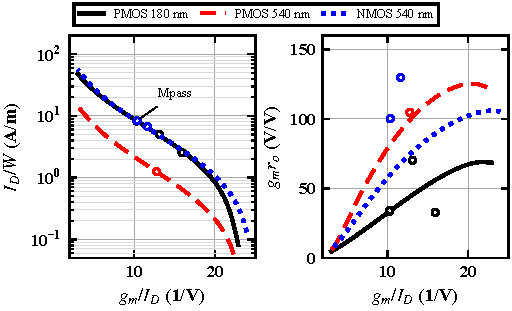
\includegraphics[width=\columnwidth]{techplot}
\caption{Techplot curves at $|V_{DS}|=0.4$~V used for sizing, with the simulated operating point of each transistor (circles). The $g_mr_o$ points differ from the curves where the device's actual $|V_{DS}|$ is not 0.4~V.}
\label{fig:techplot}
\end{figure}

\begin{table}[!t]
\centering
\caption{Transistor sizes and simulated operating point (1.8 V, 10 mA)}
\label{tab:sizing}
\footnotesize
\setlength{\tabcolsep}{1.6pt}
\begin{tabular}{@{}llcccc@{}}
\toprule
Device & Role & $W$ ($\mu$m) / $L$ & $I_D$ & $g_m/I_D$ & $g_mr_o$ \\
\midrule
M$_{\rm PASS}$ & Pass device & 1223 / 180 nm & 10.15 mA & 10.3 & 34 \\
M$_{\rm REF}$ & Mirror reference & 12.229 / 180 nm & 101.3 $\mu$A & 10.3 & 34 \\
M$_{\rm C}$ & Cascode ($r=V_{\rm OUT}$) & 40 / 180 nm & 101.3 $\mu$A & 15.9 & 33 \\
M$_{\rm CN}$ & Driver cascode & 20 / 540 nm & 134.2 $\mu$A & 11.6 & 130 \\
M$_{\rm DRV}$ & Driver & 24 / 1 $\mu$m & 134.2 $\mu$A & 8.7 & 17 \\
M$_{\rm PI1,2}$ & EA input pair & 20 / 540 nm & 25.0 $\mu$A & 12.8 & 105 \\
M$_{\rm NL1,2}$ & EA mirror load & 3 / 540 nm & 25.0 $\mu$A & 10.4 & 100 \\
M$_{\rm FO}$ & Follower ($V_{\rm OUT}$) & 4 / 180 nm & 20.0 $\mu$A & 19.4 & 35 \\
M$_{\rm FR}$ & Follower ($r$) & 4 / 180 nm & 20.0 $\mu$A & 19.4 & 35 \\
M$_{1,2}$ & Tracking pair & 12 / 180 nm & 30.1 $\mu$A & 21.1 & 34 \\
M$_{\rm L1,2}$ & Tracking load & 6 / 180 nm & 30.1 $\mu$A & 13.1 & 70 \\
\midrule
M$_{\rm SP}$ & Start-up detector & 1 / 4 $\mu$m & 16 nA & -- & -- \\
M$_{\rm SN,SD}$ & Start-up detector & 2 / 540 nm & 16 nA & -- & -- \\
M$_{\rm KU}$ & Start-up kick & 0.5 / 4 $\mu$m & off & -- & -- \\
\bottomrule
\end{tabular}
\end{table}

\begin{table}[!t]
\centering
\caption{Quiescent-current budget (1.8 V, 10 mA)}
\label{tab:budget}
\footnotesize
\begin{tabular}{@{}lc@{}}
\toprule
Branch & Current ($\mu$A) \\
\midrule
Mirror reference ($I_D/N$) & 101.6 \\
$R_G$ (gate pull-up) & 32.9 \\
Error-amplifier tail & 50.0 \\
Tracking followers (2$\times$) & 40.0 \\
Tracking pair tails (2$\times$) & 60.0 \\
Feedback divider & 5.0 \\
\midrule
Sum of branches & 289.5 \\
Simulated (supply $-$ load) & 289.2 \\
\bottomrule
\end{tabular}
\end{table}


Table~\ref{tab:budget} shows where the 289~$\mu$A goes; the sum of the designed branch currents matches the simulated supply current to within 0.3~$\mu$A.

\section{Compensation and Stability}
\subsection{Output-pole-dominant loop}
The loop gain is measured with an AC source in series with the gate of the error amplifier's input transistor. Since a gate draws no current, this breaks the loop exactly at every load, including no load. The 891-pF output capacitor sets the dominant pole. The $R_Z$--$C_Z$ network at the OTA output adds a lag--lead zero at $1/(2\pi R_ZC_Z)=398$~kHz, above which the OTA gain is $g_{m,\rm in}R_Z$. The driver current is mirrored by $N_{\rm eff}=g_{m,\rm PASS}/(g_{m,\rm REF}+1/R_G)\approx 95$, so the crossover is
\begin{equation}
f_u \approx \frac{g_{m,\rm in}\,R_Z\,g_{m,\rm DRV}\,N_{\rm eff}}{2\pi\,\Cout} \approx 26~{\rm MHz},
\end{equation}
against 21.4~MHz in simulation. The hand estimate ignores the gate pole, which explains most of the 24\% error.

\subsection{Feed-forward capacitor across the divider}
At first the crossover was only 6~MHz and the load-step error was $\pm$47~mV. The step error is roughly $\Delta V\approx\Delta I/(2\pi f_u\Cout)$, so $\pm$20~mV needs $f_u\approx 18$~MHz. Raising $R_Z$ alone ran into the pole at the divider tap (64~k$\Omega$ driving the input gate). An 8-pF capacitor $C_{FF}$ across $R_T$ makes $\beta\to1$ above $1/(2\pi R_TC_{FF})=110$~kHz. This removes the divider pole, nearly triples the high-frequency loop gain, and also stops the divider resistors and the OTA from being amplified by $1/\beta=2.8$ in the noise. With $R_Z=4$~k$\Omega$ the crossover reaches 21~MHz with 60$^\circ$ phase margin at 10~mA (Fig.~\ref{fig:loop}).

\subsection{Light load: the gate pole and $R_G$}
The second pole is at the gate node, $f_g=g_{m,\rm REF}/(2\pi C_g)\approx 53$~MHz at 10~mA. At light load, however, $I_{\rm REF}=I_{\rm PASS}/100$ falls to about 2~$\mu$A and M$_{\rm REF}$ goes into subthreshold. $f_g$ then drops to about 2~MHz, right onto the crossover, and the phase margin fell to 18$^\circ$. A 20-k$\Omega$ resistor $R_G$ from $\Vin$ to the gate sets a load-independent floor on the gate conductance. Its 33~$\mu$A is not mirrored, because it does not flow through M$_{\rm REF}$. Since the gate follows $\Vin$, very little ripple flows through it. Fig.~\ref{fig:pm} shows the result: at least 48.9$^\circ$ from no load to 10~mA at both line extremes, with 75--85~dB of DC loop gain everywhere.

\begin{figure}[!t]
\centering
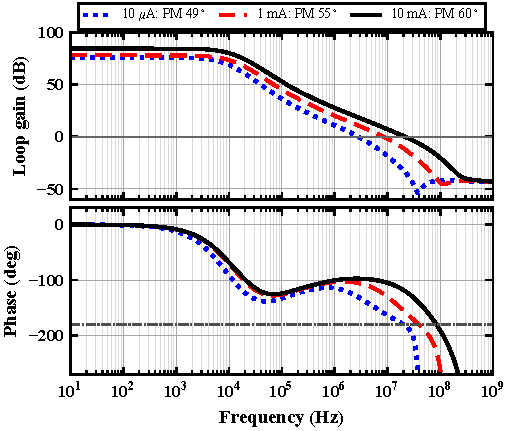
\includegraphics[width=\columnwidth]{loop_gain}
\caption{Loop gain and phase at 1.89~V (the worst line for phase margin) at three load currents.}
\label{fig:loop}
\end{figure}

\begin{figure}[!t]
\centering
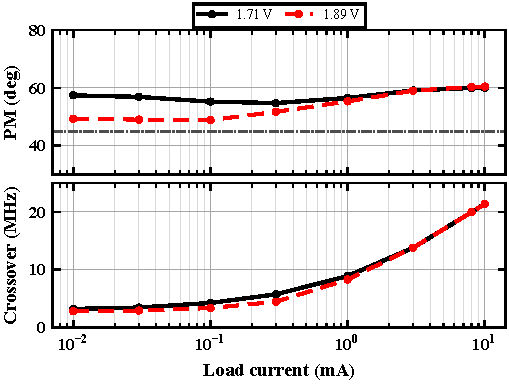
\includegraphics[width=\columnwidth]{pm_vs_load}
\caption{Phase margin and crossover frequency versus load current at the two line extremes. The dash-dot line marks 45$^\circ$.}
\label{fig:pm}
\end{figure}

\section{Simulation Results}
Table~\ref{tab:results} summarizes the performance; every entry meets its target.

\begin{table}[!t]
\centering
\caption{Simulated performance against the specification}
\label{tab:results}
\footnotesize
\setlength{\tabcolsep}{2pt}
\begin{tabular}{@{}lccc@{}}
\toprule
Parameter & Target & NCM-LDO & Status \\
\midrule
Input range & 1.71--1.89 V & 1.71--1.89 V & \textbf{Met} \\
$V_{\rm OUT}$, 0--10 mA, all $V_{\rm IN}$ & 1.4 V $\pm$1\% & 1.3997--1.4067 V & \textbf{Met} \\
Line regulation (10 mA) & -- & 0.02 mV & -- \\
Load regulation 8$\to$10 / 0$\to$10 mA & -- & 0.95 / 7.0 mV & -- \\
Dropout at 10 mA & $\le$300 mV & 25 mV & \textbf{Met} \\
Worst PSRR, 10 kHz--1 GHz\textsuperscript{a} & $\le-30$ dB & -31.3 dB & \textbf{Met} \\
Quiescent current\textsuperscript{b} & $\le$300 $\mu$A & 289 $\mu$A & \textbf{Met} \\
Total capacitance & $\le$1 nF & 1000 pF & \textbf{Met} \\
Phase margin, 0--10 mA & $\ge45^\circ$ & 48.9$^\circ$ min & \textbf{Met} \\
Noise at 1 MHz & $\le$20 nV/$\sqrt{\rm Hz}$ & 18.4 nV/$\sqrt{\rm Hz}$ & \textbf{Met} \\
Load step 8$\leftrightarrow$10 mA, 10 ns & $\pm$20 mV & $\pm$17.0 mV & \textbf{Met} \\
Line step 1.71$\leftrightarrow$1.89 V, 10 ns & -- & -2.0 / +2.1 mV & -- \\
\bottomrule
\end{tabular}

\vspace{2pt}
\parbox{\columnwidth}{\scriptsize LTspice, typical models, 27$^\circ$C, ideal reference and bias sources.
\textsuperscript{a}Over 1.71/1.8/1.89 V, 8/10 mA, current-source and resistive loads (12 cases).
\textsuperscript{b}At 1.8 V, 10 mA; supply current minus load current.}
\end{table}


\textbf{PSRR.} Fig.~\ref{fig:envelope} shows the worst case over all 12 line, load and load-type combinations from 10~Hz to 10~GHz. Below 10~kHz the PSRR is $-76$ to $-84$~dB, and at 10~GHz it is back to $-60$~dB. In between it is $-56$ to $-65$~dB at 100~kHz, $-51$ to $-59$~dB at 1~MHz and $-41$ to $-46$~dB at 10~MHz. It then levels off at about $-32$~dB between 40 and 400~MHz. The worst point is $-31.3$~dB (1.71~V, 10~mA, 42~MHz). Compared with the conventional LDO in Fig.~\ref{fig:conv}, the hump at 3.5~MHz is gone, an improvement of about 50~dB there.

\textbf{Gain.} The DC loop gain is 75--85~dB at every load from 0 to 10~mA (Fig.~\ref{fig:loop}). The error amplifier alone gives about 35~dB (hand estimate 33~dB in the design sheet), and the driver, mirror and output stage give the rest. At 10~mA the loop crosses over at 21.4~MHz.

\begin{figure}[!t]
\centering
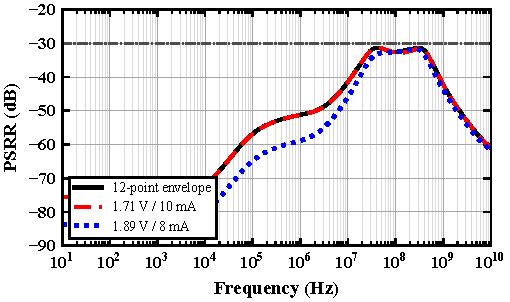
\includegraphics[width=\columnwidth]{psrr_envelope}
\caption{Pointwise worst PSRR over 1.71/1.8/1.89~V, 8/10~mA and current-source/resistive loads, with two individual cases.}
\label{fig:envelope}
\end{figure}

\textbf{Transient response.} Fig.~\ref{fig:loadstep} shows the 8$\leftrightarrow$10-mA load step: the output moves by 17~mV and recovers. The fast part follows the 21-MHz loop; the slower tail (about 3~$\mu$s to settle within 1~mV) comes from the low-frequency doublets created by $C_{FF}$ and $C_Z$. A 1.71$\leftrightarrow$1.89-V line step in 10~ns disturbs the output by only $-2.0$/$+2.1$~mV (Fig.~\ref{fig:linestep}).

\begin{figure}[!t]
\centering
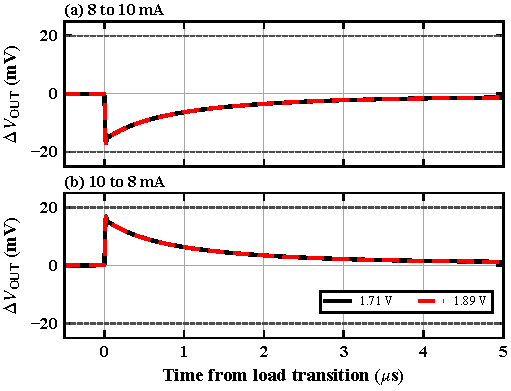
\includegraphics[width=\columnwidth]{load_step}
\caption{Load-step response at both line extremes: (a) 8 to 10~mA and (b) 10 to 8~mA, 10-ns edges. Dashed lines mark the $\pm$20-mV limit.}
\label{fig:loadstep}
\end{figure}

\begin{figure}[!t]
\centering
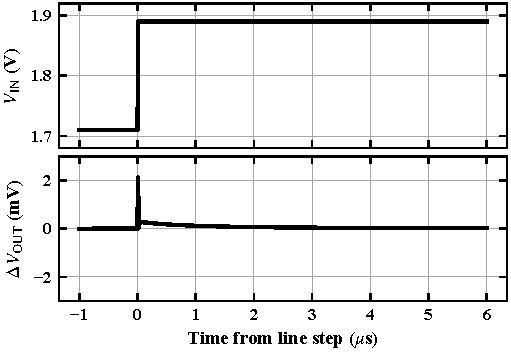
\includegraphics[width=\columnwidth]{line_step}
\caption{Line step from 1.71 to 1.89~V in 10~ns at 10~mA.}
\label{fig:linestep}
\end{figure}

\textbf{Noise.} The output noise is 18.4~nV/$\sqrt{\rm Hz}$ at 1~MHz and 112~$\mu$V$_{\rm rms}$ from 1~kHz to 100~MHz (Fig.~\ref{fig:noise}). Before $C_{FF}$ was added it was 105~nV/$\sqrt{\rm Hz}$, because the divider and the OTA noise were amplified by $1/\beta$.

\begin{figure}[!t]
\centering
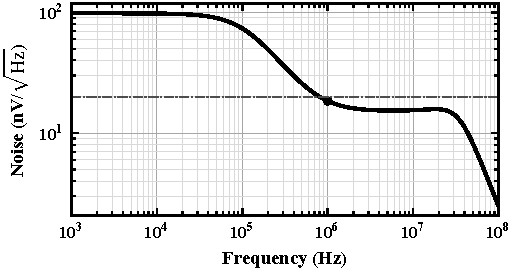
\includegraphics[width=\columnwidth]{noise}
\caption{Output noise density at 1.8~V, 10~mA. The dash-dot line marks the 20-nV/$\sqrt{\rm Hz}$ target at 1~MHz.}
\label{fig:noise}
\end{figure}

\textbf{Start-up.} I ramped $\Vin$ from 0~V to 1.71 and 1.89~V in 0.1, 10 and 100~$\mu$s, with a 140-$\Omega$ load, a 10-mA load and no load, starting from an all-zero state. All bias sources were made compliant: they scale with $\Vin$ and with the voltage across them, as a real bias generator would. All 18 cases start and settle to 1.40~V. With a load, the output rises monotonically with no overshoot. Without a load there are dips of at most 18~mV on the fast ramps, and the peak is 1.407~V. Fig.~\ref{fig:startup} shows two cases: after a fast ramp the output settles within about 13~$\mu$s; on a slow ramp it stays at 0 until $\Vin\approx1.35$~V and then follows the supply up to 1.40~V.

\begin{figure}[!t]
\centering
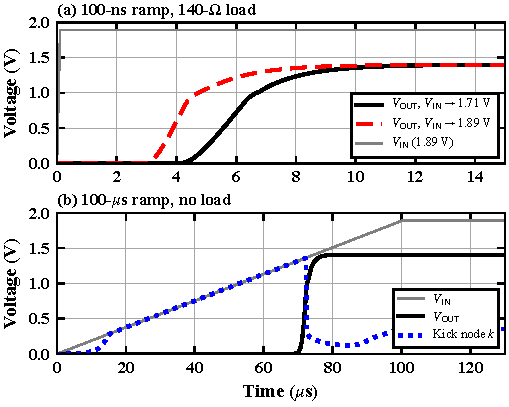
\includegraphics[width=\columnwidth]{startup}
\caption{Power-up from 0~V: (a) 100-ns supply ramp to both line extremes with a 140-$\Omega$ load; (b) 100-$\mu$s ramp with no load, showing the kick node $k$.}
\label{fig:startup}
\end{figure}

\section{Limitations}
\textbf{The 40--400-MHz floor.} The PSRR does not have a peak that could be notched out; it has a flat floor near $-32$~dB. Fig.~\ref{fig:tracking} shows why. Above about 30~MHz the tracking amplifier can no longer hold $r$ at $\Vout$. The gate of M$_{\rm C}$ then follows $r$ through its $C_{gs}$, so M$_{\rm C}$'s effective transconductance collapses. The neutralizing current through $C_N$ arrives with the wrong phase, and the gate stops following $\Vin$ (the gate error rises from $-33$~dB to $-6$~dB). The neutralization path is fundamentally limited near
\begin{equation}
f_{\rm ceil}\approx \frac{g_{m,\rm C}}{2\pi C_N}\approx 265~{\rm MHz}.
\end{equation}
Pushing this floor down needs a faster tracking amplifier or a buffered cascode gate, and both cost current that the 300-$\mu$A budget does not have. Spending 100~$\mu$A more on the reference current improves the floor by only about 1.6~dB.

\textbf{Light load at high line.} The PSRR specification applies at 8--10~mA. At 1.89~V and below 1~mA, the gate voltage $\Vin-V_{SG}$ rises close to $\Vout$, M$_{\rm C}$ runs out of headroom and $r$ stops tracking $\Vout$. The PSRR there degrades to $-19$ to $-25$~dB, although the loop stays stable.

\textbf{Not verified.} Process corners, mismatch (the cancellation depends on matching M$_{\rm REF}$ to M$_{\rm PASS}$ and $C_N$ to $\Cgd$), temperature, and a real reference and bias circuit were not simulated (the start-up test models the bias generators behaviorally). $C_N$ is the most sensitive component: 0.90~pF instead of 1.00~pF already gives $-28.5$~dB.

\begin{figure}[!t]
\centering
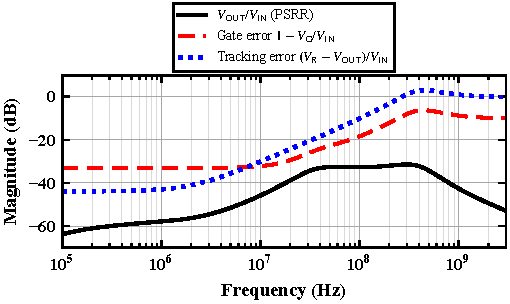
\includegraphics[width=\columnwidth]{tracking}
\caption{Origin of the PSRR floor (1.89~V, 10~mA, 1-V supply ripple): above about 30~MHz node $r$ stops tracking $\Vout$ and the gate stops following $\Vin$.}
\label{fig:tracking}
\end{figure}

\section{Conclusion}
I designed a neutralized current-mode LDO in 180-nm CMOS that regulates 1.8~V down to 1.4~V for an on-chip PLL. Using the pass device as a 100$\times$ mirror with its reference drain held at $\Vout$ cancels the $g_m$ and $g_{ds}$ ripple paths. A 1-pF capacitor injected at the reference drain cancels the $\Cgd$ path, which the mirror would otherwise multiply by 100. With $g_m/I_D$ sizing from the techplots, the simulated regulator meets every specification in Table~\ref{tab:specs}: $-31.3$~dB worst-case PSRR from 10~Hz to 10~GHz, 289~$\mu$A, exactly 1~nF, 25-mV dropout, at least 48.9$^\circ$ phase margin from no load to full load, 18.4~nV/$\sqrt{\rm Hz}$ and $\pm$17-mV load-step error. A four-transistor kick on the error-amplifier output gives clean start-up from 0~V.

The remaining PSRR floor is set by how fast the neutralizing current can be delivered into the gate node. Lowering it means spending more current, which for an on-chip LDO at this node soon stops being worth it. I therefore stopped the design at this point. The next steps would be corner and mismatch verification, and a real reference and bias circuit.

\begin{thebibliography}{9}
\bibitem{adi} S.~Iriarte and A.~Marinas, ``High power supply rejection ratio (PSRR) and low dropout regulator,'' U.S. Patent 8\,928\,296 B2, Jan. 6, 2015 (Analog Devices, Inc.).
\bibitem{park} C.-J.~Park, M.~Onabajo, and J.~Silva-Martinez, ``External capacitor-less low drop-out regulator with 25 dB superior power supply rejection in the 0.4--4 MHz range,'' \emph{IEEE J. Solid-State Circuits}, vol.~49, no.~2, 2014.
\bibitem{lim} Y.~Lim \emph{et al.}, ``An external capacitorless low-dropout regulator with high PSR at all frequencies from 10 kHz to 1 GHz using an adaptive supply-ripple cancellation technique,'' \emph{IEEE J. Solid-State Circuits}, vol.~53, no.~9, pp.~2675--2685, 2018.
\bibitem{elnozahi} M.~El-Nozahi \emph{et al.}, ``High PSR low drop-out regulator with feed-forward ripple cancellation technique,'' \emph{IEEE J. Solid-State Circuits}, vol.~45, no.~3, pp.~565--577, 2010.
\bibitem{choe} Y.-J.~Choe, H.~Nam, and J.-D.~Park, ``A low-dropout regulator with PSRR enhancement through feed-forward ripple cancellation technique in 65 nm CMOS process,'' \emph{Electronics}, vol.~9, no.~1, p.~146, 2020.
\end{thebibliography}
\end{document}
